\documentclass[]{scrartcl}
\usepackage{graphicx}
\usepackage{geometry}
\geometry{
	a4paper,
	total={170mm,257mm},
	left=20mm,
	top=20mm,
}


%opening
\title{SDD -Client Low Level Design}
\author{Brandon Smith, Nieka Gutenberger, Joseph Coppin, Ryan Frazier, Trevor Jewkes}

\begin{document}

\maketitle

\centerline{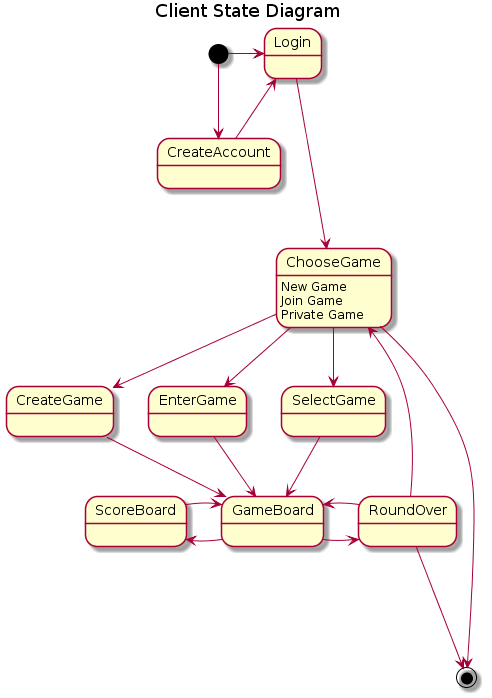
\includegraphics{Client State Diagram.png}}
\noindent\makebox[\textwidth{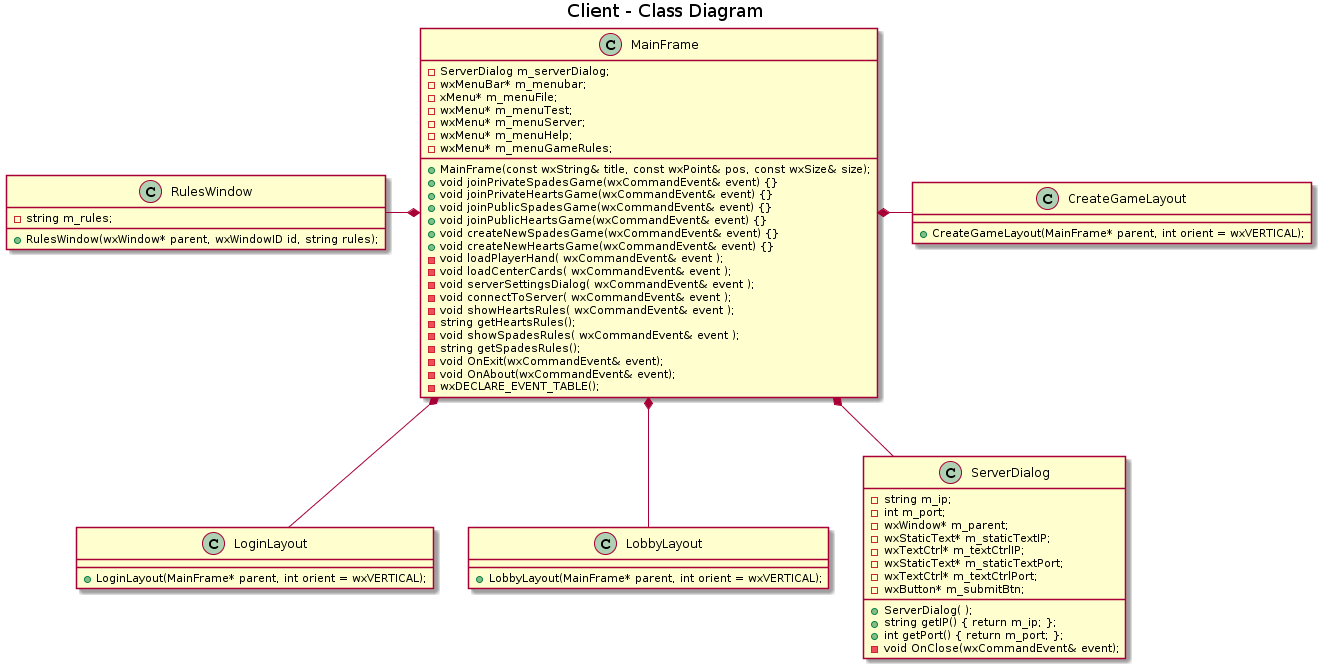
\includegraphics[width=\textwidth]{clientClassDiagram.png}}]

\section{MainFrame}
	This class is inherited publically from wxFrame.

	\begin{itemize}
		\item public:

		\begin{itemize}
			\item MainFrame(const wxString\& title, const wxPoint\& pos, const wxSize\& size);
				\\ In the main frame, the main components of the software are held. Following are the functions included:

			\item void joinPrivateSpadesGame(wxCommandEvent\& event) {}
				\\This function allows a user to join a spades game that is closed to public use.

			\item void joinPrivateHeartsGame(wxCommandEvent\& event) {}
				\\ This function allows a user to join a hearts game that is closed to public view.

			\item void joinPublicSpadesGame(wxCommandEvent\& event) {}
				\\ This function will allow user to connect to first available spades game.

			\item void joinPublicHeartsGame(wxCommandEvent\& event) {}
				\\ This function will allow user to connect to first available hearts game.

			\item void createNewSpadesGame(wxCommandEvent\& event) {}
				\\	This function will create a new Spades Game.

			\item void createNewHeartsGame(wxCommandEvent\& event) {}
				\\ This function will create a new Hearts Game.

		\end{itemize}

		\item 	private:

		\begin{itemize}
			\item ServerDialog m\_serverDialog;
			\item wxMenuBar* m\_menubar;
			\item xMenu* m\_menuFile;
			\item wxMenu* m\_menuServer;
			\item wxMenu* m\_menuHelp;
			\item wxMenu* m\_menuGameRules;
			\item void loadPlayerHand( wxCommandEvent\& event );
				\\Allows for players hand to be loaded on screen from server.
			\item void loadCenterCards( wxCommandEvent\& event );
				\\Allows for cards to be placed in middle of screen after play.
			\item void serverSettingsDialog( wxCommandEvent\& event );
			\item void connectToServer( wxCommandEvent\& event );
				\\Allows player to connect to server to play game of choice.
			\item void showHeartsRules( wxCommandEvent\& event );
				\\Allows user to get Hearts Rules.
			\item std::string getHeartsRules();
			\item void showSpadesRules( wxCommandEvent\& event );
				\\Allows user to get Spades Rules.
			\item std::string getSpadesRules();
			\item void OnExit(wxCommandEvent\& event);
				\\Allows user to exit program.
			\item void OnAbout(wxCommandEvent\& event);
				\\Allows user to see details of program.
			\item wxDECLARE\_EVENT\_TABLE();
		\end{itemize}
	\end{itemize}


\section{ServerDialog }
	This class is inherited publically from wxDialog.
	\begin{itemize}
	\item public:

	\begin{itemize}
		\item ServerDialog( wxWindow* parent, wxWindowID id = wxID\_ANY, const wxString\& title = wxEmptyString, const wxPoint\& pos = wxDefaultPosition, const wxSize\& size = wxDefaultSize, long style = wxDEFAULT\_DIALOG\_STYLE );

		\item std::string getIP() { return m\_ip; };

		\item int getPort() { return m\_port; };
	\end{itemize}

	\item private:
	\item protected:
		\begin{itemize}
			\item std::string m\_ip;
			\item	int m\_port;
			\item	wxWindow* m\_parent;
			\item	wxStaticText* m\_staticTextIP;
			\item	wxTextCtrl* m\_textCtrlIP;
			\item	wxStaticText* m\_staticTextPort;
			\item	wxTextCtrl* m\_textCtrlPort;
			\item	wxButton* m\_submitBtn;
			\item	void OnClose(wxCommandEvent\& event);
		\end{itemize}
	\end{itemize}

\section{RulesWindow }
	This class is inherited  publically from wxScrolledWindow

	\begin{itemize}
		\item 	public:
		\begin{itemize}
			\item RulesWindow(wxWindow* parent, wxWindowID id, std::string rules);
				\\This allows user to read and learn rules for either Hearts or Spades.
		\end{itemize}
	\end{itemize}

	\begin{itemize}
		\item 	private:
		\begin{itemize}
			\item std::string m\_rules;
		\end{itemize}
	\end{itemize}


\section{LoginLayout }
	This class is inherited  publically from wxBoxSizer
	\begin{itemize}
		\item public:
		\begin{itemize}
			\item	LoginLayout(MainFrame* parent, int orient = wxVERTICAL);
				\\This function will bring up a screen where user may login to play game.
		\end{itemize}
	\end{itemize}



\section{LobbyLayout}
	This class is inherited  publically from wxBoxSizer
		\begin{itemize}
			\item public:
			\begin{itemize}
				\item	LobbyLayout(MainFrame* parent, int orient = wxVERTICAL);
					\\This function allows the user to access the game lobby.
			\end{itemize}
		\end{itemize}

\section{CreateGameLayout}
	This class is inherited  publically from wxBoxSizer

		\begin{itemize}
			\item public:
			\begin{itemize}
				\item	CreateGameLayout(MainFrame* parent, int orient = wxVERTICAL);
					\\When called, this function sets up a game layout for game play.
			\end{itemize}
		\end{itemize}

\end{document}
